\documentclass[12pt, twoside]{article}
\usepackage[francais]{babel}
\usepackage[T1]{fontenc}
\usepackage[latin1]{inputenc}
\usepackage[left=7mm, right=7mm, top=8mm, bottom=8mm]{geometry}
\usepackage{float}
\usepackage{graphicx}
\usepackage{array}
\usepackage{multirow}
\usepackage{amsmath,amssymb,mathrsfs}
\usepackage{textcomp}
\pagestyle{empty}
\usepackage{soul}
\begin{document} 

NOM: \\
PRENOM: 

\bigskip


\begin{center}
{\fbox{$2^{de}5$ \qquad \qquad \textbf{\Large{Devoir surveill� 4}}
\qquad \qquad 20/12/2008}}
\end{center}

\textit{On rappelle qu'en g�om�trie ``voir sur la figure'' n'est pas une
d�monstration. L'exercice 5 doit �tre trait� en dernier.}

\bigskip


\textbf{Exercice 1:}


\begin{tabular}{cc}
\begin{minipage}{6cm}
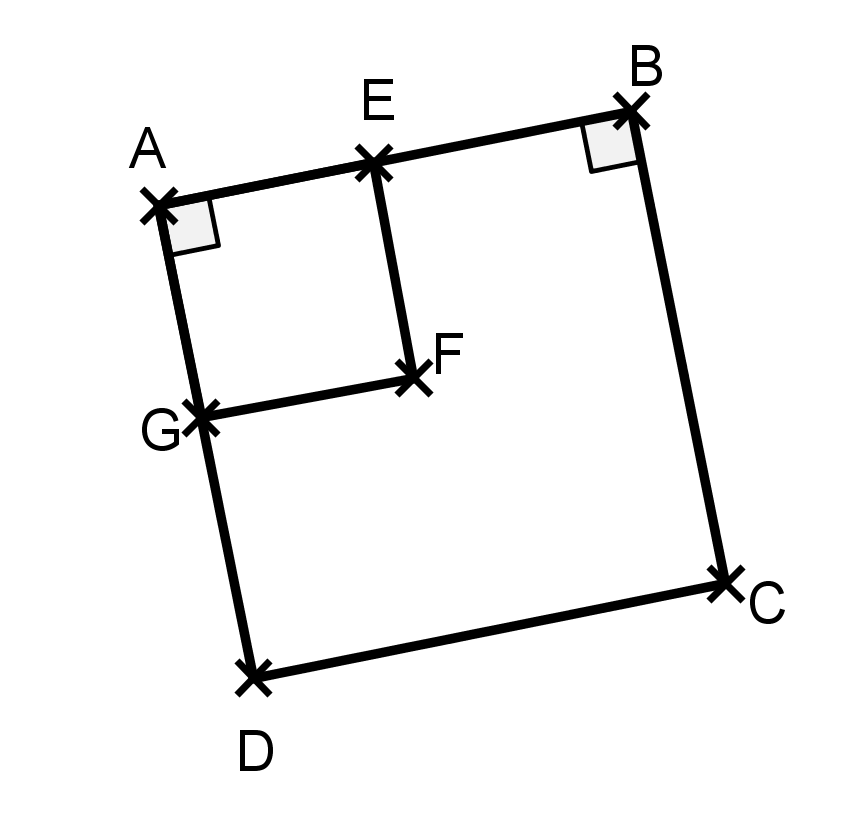
\includegraphics[width=6cm]{images/ex1.png}
\end{minipage}
&
\begin{minipage}{12cm}
 Soit $\mathcal{C}$ un cercle de centre $O$ et de diam�tre
$[AB]$. $D$ et $C$ sont deux points de ce cercle, $\widehat{BOC}=30$� et
$\widehat{OAD}=45$�.
\begin{enumerate}
  \item Que peut-on dire du triangle $AOD$? Justifier votre r�ponse.
  \item Que peut-on dire du triangle $OCD$? Justifier votre r�ponse. 
\end{enumerate}
\end{minipage}
\end{tabular}

\bigskip
\bigskip
 
 \textbf{Exercice 2:} R�soudre les �quations suivantes:
 
 $2x+3=0$
 
 \enskip
 
  $2(x-7)=(x-7)(3+2x)$
  
 \enskip

  $\dfrac{3-4x}{x-7}=0$

\enskip


$81x^{2}+36x+4=0$
 


 
 \bigskip
 \bigskip
 
 \textbf{Exercice 3:} \textit{La premi�re question est � faire sur la feuille,
 la deuxi�me sur votre copie.}
 \bigskip
 
 \begin{enumerate}
   \item 

 $\begin{array}{|c|ccccc|}
\hline
 x & -\infty & \ \ \ \ \ \ \ \ \ \ \ & 4 &\ \ \ \ \  \ \ \ \ \ & +\infty \\
 \hline
2x-8 & \ \ & - & \ \ \ \ 0 \ \ \ \ & + & \ \ \\
 \hline
 \end{array}$
 
\begin{enumerate}
  \item Compl�ter les phrases:
  
   
     Pour $x$ \ldots \ldots , $2x-8$ est positif. 
     
     Pour $x=\ldots
  \ldots$, $2x-8$ est nul. 
  
  
  Pour $x<4$, $2x-8$ est \ldots \ldots \ldots \ldots
  
  \enskip
 
  \item Quel est le signe de $2x-8$ pour $x=6$? \rule{100mm}{0.5pt}
  
  
  Quel est le signe de $2x-8$ pour $x=-1$? \rule{100mm}{0.5pt}
  
  
  
Quel est le signe de $2x-8$ pour $x=-4$? \rule{100mm}{0.5pt}
\end{enumerate}





\item R�soudre l'in�quation suivante: $(2x+3)(2-x) \leqslant 0$.
\end{enumerate}


\bigskip
\bigskip

\textbf{Exercice 4:} Indiquer pour chaque expression s'il s'agit d'une somme,
d'un produit ou d'un quotient puis d�velopper les produits, factoriser les
sommes et simplifier les quotients.

\medskip

$A=(2x+3)(2-x)$ \qquad \qquad \qquad $B=x^{2}-81$ \qquad \qquad \qquad
$C=\dfrac{(x-1)(4x-1)}{16x^{2}-8x+1}$

\pagebreak


\textbf{Exercice 5:} Soit $ABC$ un triangle �quilat�ral. Le cercle $(C)$ de
diam�tre $[AB]$ et de centre $O$, recoupe $[BC]$ en $I$. $K$ est le sym�trique
de $O$ par rapport � $B$.

\begin{center}
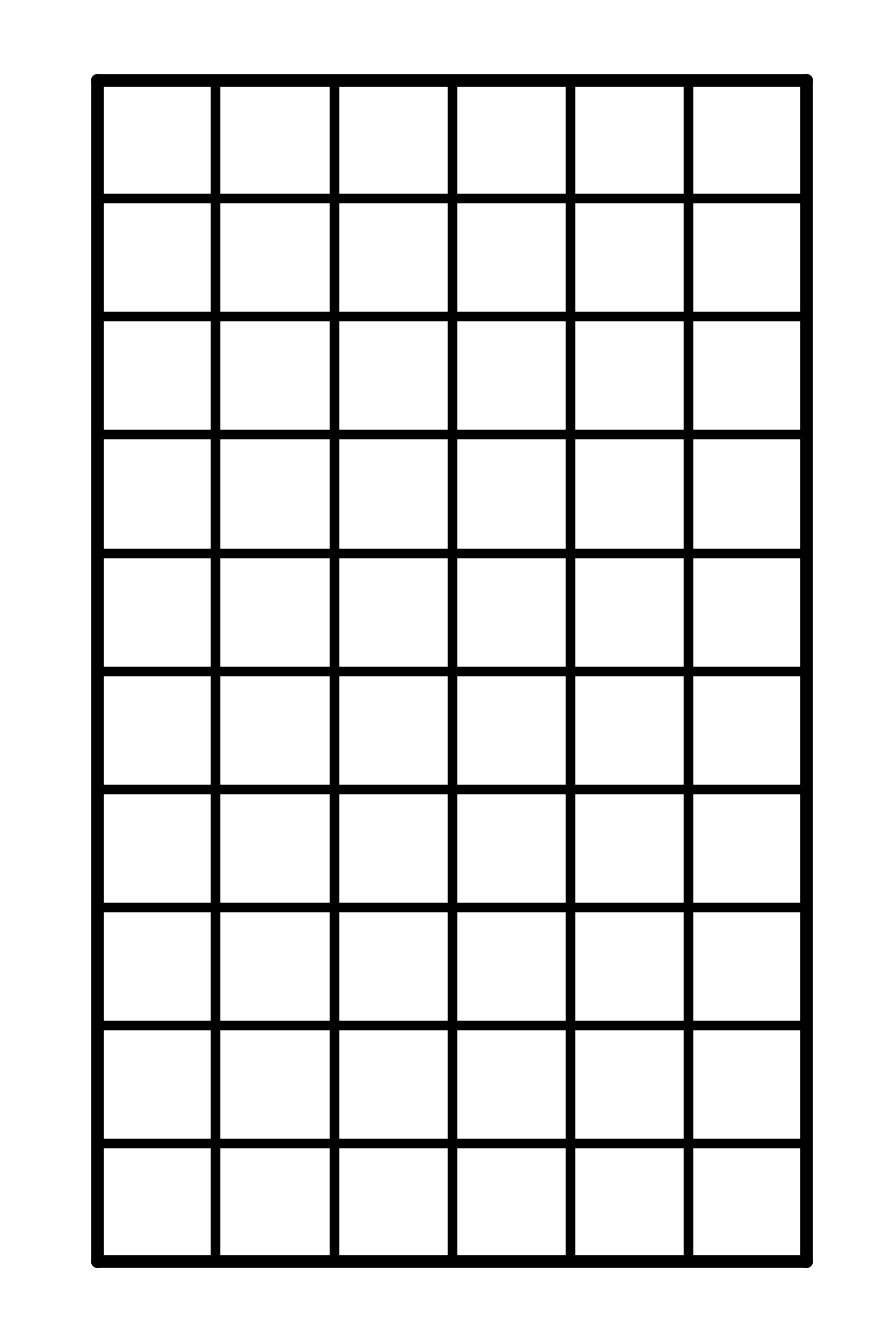
\includegraphics[width=10cm]{images/ex5.png}
\end{center}

\begin{enumerate}
  \item D�montrer que $I$ est le milieu de $[BC]$.
  \item D�montrer que les droites $(IK)$ et $(OI)$ sont perpendiculaires et en
  d�duire que les droites $(IK)$ et $(AC)$ sont perpendiculaires.
  \item \begin{enumerate}
          \item Quel est la nature du triangle $AIK$? Justifier.
          \item \ul{BONUS}: La droite $(KI)$ coupe $(CA)$ en $L$. On suppose de
          plus que $AC=4$. Calculer $IL$.
        \end{enumerate}
\end{enumerate}


\bigskip
\bigskip

\ul{THE BEST BONUS}: Soit $A=8$, $B=9$, $C=10$ \ldots

D�crypter le message suivant: $ 9 \ 22\ 21 \ 21 \ 12 \ 26$ \quad $29 \ 8 \ 10 \
8 \ 21 \ 10 \ 12 \ 26 $
\end{document}
